\chapter{Background}
\label{Background}
\section{RoboCup}
The RoboCup competition was initially inspired by Hiroaki Kitano~\cite{robocup} in 1993 and then his idea led to the foundation of the RoboCup Federation. The RoboCup competition has a bold vision:``By the year 2050, to develop a team of fully autonomous humanoid robots that can win against the human world soccer champions''. All the teams that participate in RoboCup have to find solutions to some of the most difficult problems, that the robot community has to solve, in real time (perception, cognition, action, co-ordination). All the competitions in RoboCup (soccer, RoboCup@Home, RoboRescue etc.) are testing the solutions that teams find for the problems above. So far, the researchers that participate in RoboCup have made a lot of progress to solve real-world problems that are presented through the RoboCups competitions.

\subsection{The Standard Platform League}
The Standard Platform League (SPL) is one of the soccer leagues of RoboCup. In this league all the teams use the same robot, Aldebaran-NAO, and they focus only in the software. The teams are prohibited to make any changes to the hardware of the robot, so that everyone use the same platform and compete only in software. The robots are complete autonomous and no human interaction, from the team members, is allowed during the games. The only interaction with the outer world, that robots have, is the data that Game Controller sends, which declare the state of the game.
Current the games are conducted in a field with dimensions \(4m \times 8m\)~\cite{SPLrules2012}. The field is consists from a green carpet with white lines and 2 yellow goals. The appearance of the field is similar with the real soccer field but it is scaled. The ball is a polished orange street hokey ball. Each team consists of four robots and each robot has a band, the color of the band defines the team (blue or pink). The total game time is twenty minutes and it is broken in two half, its of them has a duration of 10 minutes.
\begin{figure}[h]
	\begin{center}
		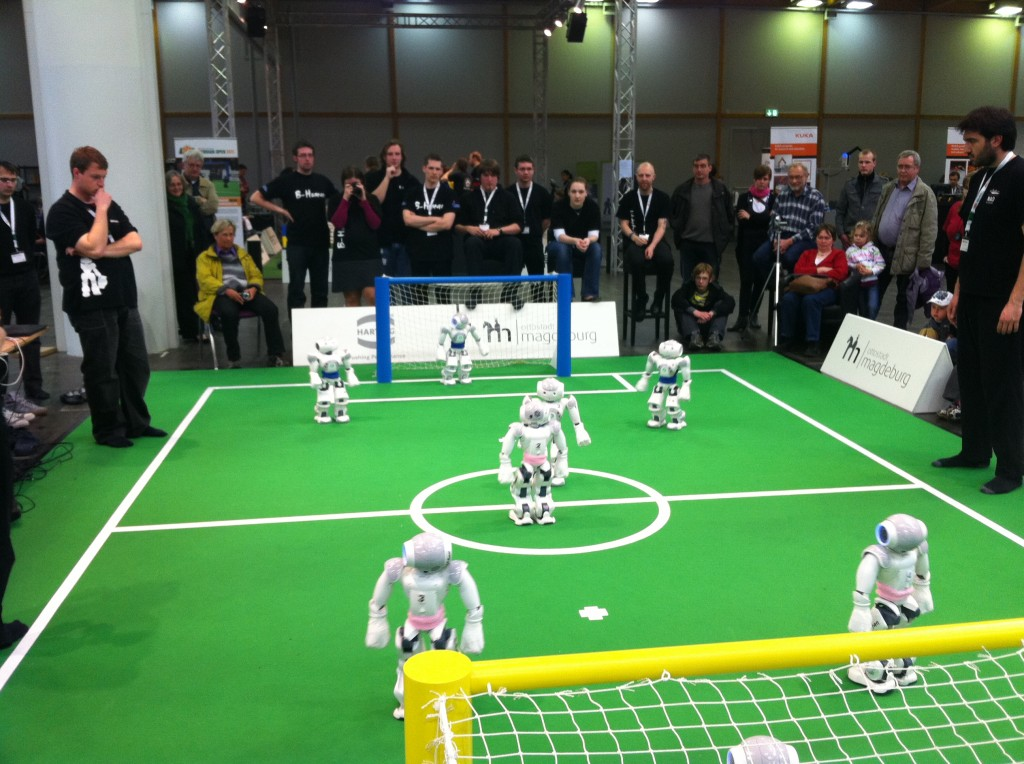
\includegraphics[height = 8cm]{Figures/RoboCupSpl.jpg}
 		\caption{RoboCup Standar Platform League}
 		\label{fig:RoboCup SPL}
	\end{center}
\end{figure}

\section{The Aldebaran NAO robot}
The NAO robot is the robot that is be used by all the teams in the standard platform league. NAO is complete autonomous, programmable, medium-sized humanoir robot developed by Aldebaran Robotics~\cite{naopaper}. Project NAO started in 2004. On August 2007 NAO officially replaced Sony's quadruped robot AIBO in the RoboCup SPL.\\
Nao (version V3.3) is a 58 cm and 5 Kg humanoid robot. The Nao robot carries a fully capable computer on board with an x86 AMD Geode processor at 500 MHz, 256 MB SDRAM and 2 GB flash memory running an Embedded Linux distribution. It is powered by a 6-cell Lithium-Ion battery which provides about 30 minutes of continuous operation and communicates with remote computers via an IEEE 802.11g wireless or a wired ethernet link. NAO RoboCup edition has 21 degrees of freedom; 2 in the head, 4 in each arm, 5 in each leg and 1 in the pelvis (there are two pelvis joints which are coupled together on one servo and cannot move independently). Nao, also, features a variety of sensors. Two cameras are mounted on the head in vertical alignment providing non-overlapping views of the lower and distant frontal areas, but only one is active each time and the view can be switched from one to the other almost instantaneously. Each camera is a 640 ? 480 VGA camera at 30 fps. Four sonars (two emitters and two receivers) on the chest allow Nao to sense obstacles in front of it. In addition, the Nao has a rich inertial unit, with two 2-axis gyroscope and one 3-axis accelerometer, in the torso that provide real-time information about its instantaneous body movements. Two bumpers located at the tip of each foot are simple ON/OFF switches and can provide information on collisions of the feet with obstacles. Finally, an array of force sensitive resistors on each foot delivers feedback of the forces applied to the feet, while encoders on all servos record the actual joint position at each time.
\begin{figure}[h]
	\begin{center}
		%\includegraphics[height = 8cm]{Figures/nao-sensors.jpg}
 		\caption{Sensors of NAO v3.3}
 		\label{fig:sensors}
	\end{center}
\end{figure}

\section{Kouretes Robocup SPL Team}
Kouretes is the first RoboCup team founded in Greece at the Tech-nical University of Crete in February 2006. The first participation of the team was in the Technical Challenges of Robocup 2006 in Bremen, Germany, when still the Four-Legged Sony AIBO robots were used. Next year the team participated also in the Four-Legged league of the RoboCup German Open 2007 competition in Hannover, Germany and ranked in the 7th/8th place. Months later the team's participation in the MSRS Simulation Challenge at RoboCup 2007 in Atlanta led to the placement of the team at the 2nd place worldwide. In RoboCup 2008 in Suzhou, China, Kouretes team participated and won two trophies: 1st place in the SPL-MSRS league and 3rd place in the SPL-NAO league. In 2009 the team participated both at the RoboCup German Open 2009 competition in Hannover and in RoboCup 2009 in Graz, Austria, in the SPL. In 2010 the team participated in the 1st ever RoboCup Mediterranean Open competition in Rome and in RoboCup 2010 in Singapore. In 2011, the team participated in the RoboCup German Open 2011 competition in Megdeburg, in Iran Open 2011 in Tehran and in RoboCup 2011 in Istanbul. Team Kouretes joined Team Noxious from UK to form a joint team for RoboCup 2011. The joint team won the 2nd place in the SPL Open Challenge competition with 139 points, only 3 points behind the top team. In 2012 the team Kouretes participated in the RoboCup German Open 2012 competion in Magdebug, in Iran Open 2011 in Tehran and in RoboCup 2012 in Mexico. The team, in Mexico, has succeed to qualify to the top 16 teams.
\begin{figure}[h]
	\begin{center}
		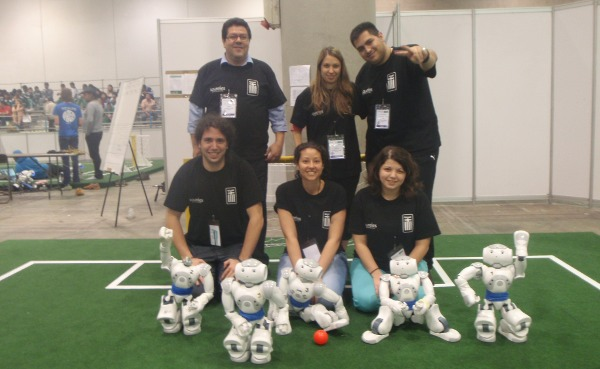
\includegraphics[height = 8cm]{Figures/robocup2012-team.jpg}
 		\caption{Kouretes team in RoboCup 2012 at Mexico City}
 		\label{fig:RoboCup2012}
	\end{center}
\end{figure}

\section{Affine Transformations}
An affine transformation is a map transferring points and vectors from one space to another, being able to preserve ratios of distances. The space can be \(n\)-dimensional with \(n\ge2\). The following are affine transformations: Geometric contraction, expansion, dilation, reflection, rotation, shear, similarity transformations, spiral similarities and translation. All the possible combinations of the above produce an affine transformation. Its flexibility concerning object manipulation, makes it a very useful tool in computer graphics.\\
For the purpose of this thesis we only used rotation and translation, so we will analyze these two types of affine transformation. Also we are working in a \(3-dimensional\) space and all the examples from now on will be in this space.\\ \\

\textbf{Affine Transformation Matrix}\\
The affine transformation matrix is a (\(n+1\times n+1\)) matrix where \(n\) is the number of dimensions. In the general form the affine transformation matrix consists of 2 parts:
\[
T = 
\begin{bmatrix}
X & Y \\
\begin{bmatrix}
0 & \cdots & 0
\end{bmatrix} & 1
\end{bmatrix}
\]
X is a (\(n\times n\)) matrix and Y is a (\(n\times 1\)) vector and the last line has \(n-1\) zeros followed by a \(1\). The matrix is invertible if and only if X is invertible and the representation of the inverse is:
\[
T = 
\begin{bmatrix}
X^{-1} & -X^{-1}Y \\
\begin{bmatrix}
0 & \cdots & 0
\end{bmatrix} & 1
\end{bmatrix}
\]
Now if we want to apply the transformation, to a given column vector \(v\), we multiply the affine transformation matrix with the given vector:
\[
v' = Tv = 
\begin{bmatrix}
X & Y \\
\begin{bmatrix}
0 & 0 & 0
\end{bmatrix} & 1
\end{bmatrix}
\begin{bmatrix}
p_x\\
p_y\\
p_z\\
1
\end{bmatrix}
\]
A matrix that is the result of \(n\) multiplications between affine transformation matrices is still an affine transformation. So in the following example, given that all the matrices in the right part of the equation are affine transformation matrices then the resulting matrix T will be an affine transformation matrix.
\[
T = T_1T_2T_3 \cdots T_n
\]

\textbf{Translation Matrix}\\
Translation, in the Euclidean space, is a function that moves every point by constant distance in a specified direction. We can describe the translation in the \(3-dimensional\) space with a (\(4\times4\)) table that has the following form:
\[
A = 
\begin{bmatrix}
1 & 0 & 0 & d_x\\
0 & 1 & 0 & d_y\\
0 & 0 & 1 & d_z\\
0 & 0 & 0 & 1
\end{bmatrix}
\]
The \(d_x,d_y,d_z\) defines the distance that we will move all of our points through the \(x,y,z\) dimension. Obviously, this is an affine transformation matrix with \(X = I\). So now if we want to apply the translation on a given column vector \(v\), we apply it in same way as the transformation:
\[
v' = Tv =
\begin{bmatrix}
1 & 0 & 0 & d_x\\
0 & 1 & 0 & d_y\\
0 & 0 & 1 & d_z\\
0 & 0 & 0 & 1
\end{bmatrix}
\begin{bmatrix}
p_x\\
p_y\\
p_z\\
1
\end{bmatrix}
\]

\textbf{Rotation Matrix}\\
Rotation matrix is a matrix that is used to perform rotation in Euclidean space. The rotation matrices are always orthogonal matrices with determinant 1.
\[R^T = R^{-1},det(R) = 1\]
In the \(3-dimensional\) Euclidean space there are three rotation matrices, each one of them makes a rotation over the \(x\)  or \(y\)  or \(z\) axis. The size of the rotation matrices, for this space, is (\(3\times3\)) and they have the following form:
\[
R_z = 
\begin{bmatrix}
\cos\theta_z & -\sin\theta_z & 0 \\
\sin\theta_z & \cos\theta_z & 0 \\
0 & 0 & 1 
\end{bmatrix}
\]
\[
R_y = 
\begin{bmatrix}
\cos\theta_y & 0 & \sin\theta_y \\
0 & 1 & 0\\
-\sin\theta_y & 0 & \cos\theta_y
\end{bmatrix}
\]
\[
R_x = 
\begin{bmatrix}
1 & 0 & 0 \\
0 & \cos\theta_x & -\sin\theta_x \\
0 & \sin\theta_x & \cos\theta_x
\end{bmatrix}
\]
Now if we want to rotate an object point, defined by the (\(3\times1\)) column vector \(v\), by the \(x\) axis and then by the \(y\) axis we will do the following:
\[
v' = R_xR_yv = 
\begin{bmatrix}
1 & 0 & 0 \\
0 & \cos\theta_x & -\sin\theta_x \\
0 & \sin\theta_x & \cos\theta_x
\end{bmatrix}
\begin{bmatrix}
\cos\theta_y & 0 & \sin\theta_y \\
0 & 1 & 0\\
-\sin\theta_y & 0 & \cos\theta_y
\end{bmatrix}
\begin{bmatrix}
p_x\\
p_y\\
p_z
\end{bmatrix}
\]
We can use combinations of those 3 matrices and make other useful rotation matrices. For example we can construct the rotation matrix that rotates all the axes with the following order, first the \(z\) axis then the \(y\) axis and finally the \(x\) axis.
\[
	R = R_zR_yR_x
\]
The analytical form of the above rotation matrix:
\[
R = 
\begin{bmatrix}
\cos\theta_y\cos\theta_z & -\cos\theta_x\sin\theta_z + \sin\theta_x\sin\theta_y\cos\theta_z & \sin\theta_x\sin\theta_z + \cos\theta_x\sin\theta_y\cos\theta_z\\

\cos\theta_y\sin\theta_z & \cos\theta_x\cos\theta_z + \sin\theta_x\sin\theta_y\sin\theta_z & -\sin\theta_x\cos\theta_z + \cos\theta_x\sin\theta_y\sin\theta_z\\

-\sin\theta_y & \sin\theta_x\cos\theta_y & \cos\theta_x\cos\theta_y
\end{bmatrix}
\]

Finally we can easily transform a rotation matrix to an affine transformation matrix just by padding with zeros and an one in the corner. So from now on whenever we use a rotation matrix, this matrix will have the following form:
\[
R' = 
\begin{bmatrix}
R &  \begin{bmatrix} 0\\0\\0 \end{bmatrix}\\
\begin{bmatrix}
0 & 0 & 0
\end{bmatrix} & 1
\end{bmatrix}
\]
\\

\textbf{Affine Transformation Matrix in this Thesis}\\
In this thesis we are using the rotation and the translation matrix so we can move points in the \(3-dimensional\) space. We can assume that our affine transformation matrix is composed by a rotation and a translation matrix. The affine transformation matrix, that we will work with, has \(X = R\) and \(Y = v\) where \(v\) is the vector with the distance points from the translation matrix.
\[
T = 
\begin{bmatrix}
R &  \begin{bmatrix} p_x\\p_y\\p_z \end{bmatrix}\\
\begin{bmatrix}
0 & 0 & 0
\end{bmatrix} & 1
\end{bmatrix}
\] 
Also we can decompose this transformation matrix to a rotation matrix followed by a translation matrix. Given a rotation \(R\) and a translation matrix \(A\):
\[R = 
\begin{bmatrix}
R &  \begin{bmatrix} 0\\0\\0 \end{bmatrix}\\
\begin{bmatrix}
0 & 0 & 0
\end{bmatrix} & 1
\end{bmatrix}
\]
\[A = 
\begin{bmatrix}
I &  \begin{bmatrix} p_x\\p_y\\p_z \end{bmatrix}\\
\begin{bmatrix}
0 & 0 & 0
\end{bmatrix} & 1
\end{bmatrix}
\]
The result from the multiplication of \(R\) with \(A\) is:
\[
T = RA = 
\begin{bmatrix}
R &  R\begin{bmatrix} p_x\\p_y\\p_z \end{bmatrix}\\
\begin{bmatrix}
0 & 0 & 0
\end{bmatrix} & 1
\end{bmatrix}
\]
So we can assume that the translation matrix \(A'\) is:
\[
A' = 
\begin{bmatrix}
I &  R\begin{bmatrix} p_x\\p_y\\p_z \end{bmatrix}\\
\begin{bmatrix}
0 & 0 & 0
\end{bmatrix} & 1
\end{bmatrix}
\]
Now if we multiply \(A'\) with the \(R\) we will have the same transformation matrix as before:
 
\[
A'R = 
\begin{bmatrix}
I &  R\begin{bmatrix} p_x\\p_y\\p_z \end{bmatrix}\\
\begin{bmatrix}
0 & 0 & 0
\end{bmatrix} & 1
\end{bmatrix}
\begin{bmatrix}
R &  \begin{bmatrix} 0\\0\\0 \end{bmatrix}\\
\begin{bmatrix}
0 & 0 & 0
\end{bmatrix} & 1
\end{bmatrix}
= 
\begin{bmatrix}
R &  R\begin{bmatrix} p_x\\p_y\\p_z \end{bmatrix}\\
\begin{bmatrix}
0 & 0 & 0
\end{bmatrix} & 1
\end{bmatrix} =
RA
\]

\section{Robot Kinematics}
Robot kinematics is the way to apply the geometry to the study of the multi-degree of freedom kinematic chains. Kinematic chain is the assembly of links connected by joints. The degree of freedom (DOF) refers to the number of joints in the kinematic chain. Robot kinematics is the way to go from the \(joint\) space, where the kinematic chains are defined, to the Euclidean space and vice versa. They are, also, very useful because we can plan and control movement and calculate actuator forces and torques.\\
\textbf{Joint Space}\\
Kinematic chain typically is a manipulator that interacts with the environment. The joints are controlling the manipulator. Not all the combinations of all joints positions in the chain are valid, because some combinations lead to collisions between the links of the chain or with some item of the environment. All the valid combinations create the \(joint\) space.
\subsection{Forward Kinematics}
The \(joint\) space reveals very little information about the position of the end effector of the kinematic chain. With the forward kinematics we can move from the \(joint\) space to the \(3-dimensional\) space. Given a kinematic chain and all the current joint values, forward kinematics can find the point \(p_x,p_y,p_z\) and the orientation \(a_x,a_y,a_z\) of the end effector of the kinematic chain. Forward kinematics is not an application specific problem and can be addressed to any kinematic chain.
\subsection{Inverse Kinematics}
Generally it is very easy for humans to give a target point or design a trajectory in \(3-dimensional\) space, but if we want the end effector to follow the trajectory, we must assign the right values to the joints of the kinematic chain. So, we need a way to go from \(3-dimensional\) space back to \(joint\) space. The problem of inverse kinematics is application specific and every kinematic chain has a different solution. The solution of the problem can be analytical or it can be approximate (e.g with Jacobian approximation method). As the DOF increases, each point in the \(3-dimensional\) space may have more than one matching point in the \(joint\) space, so we may have more than one solution in the \(joint\) space for a given point in \(3-dimensional\) space.\\

\section{DH (Denavit \- Hartenberg) Parameters}
Denavit and Hartenberg found a way to create a transformation matrix that describes points in one end of the joint to a coordinate system that is fixed to the other end, as a function of the joint state~\cite{dhparam1}~\cite{dhparam2}~\cite{introroboticscraigbook}. They found that we can construct this transformation matrix using only 4 parameters, the DH (Denavit \- Hartenberg) Parameters. These parameters are: 
\[a,\alpha,d \text{ and } \theta\]
Before we can explain these parameters we must first establish the reference frame of each joint respectively to the previous joint reference frame.
\begin{itemize}
\item The \(z_n\)-axis is in the direction of the joint axis. 
\item The \(x_n\)-axis is parallel to the common normal: \(x_n = z_n \times z_{n-1}\). The direction of \(x_n\) is from \(z_{n - 1}\) to \(z_n\).
\item The \(y_n\)-axis follows from the \(x_n\)  and \(z_n\)-axis by choosing it to be a right-handed coordinate system.
\end{itemize}
Now we can describe the DH parameters as following:
\begin{itemize}
\item\(a\): length of the common normal.
\item\(alpha\): angle about common normal, from \(z_{n-1}\)-axis to \(z_n\)-axis.
\item\(d\): offset along \(z_{n-1}\) to the common normal.
\item\(\theta\): angle about \(z_{n-1}\), from \(x_{n-1}\) to \(x_n\).
\end{itemize}
There is a great site with that explains the way to find those parameters and has some videos to visualize the explanation~\cite{tekkotsu}.
Now we can go from one reference frame to the other by composing the transformation matrix:
\[DH = R_x(\alpha)T_x(a)R_z(\theta)T_z(d)\]
The analytical form of the resulting matrix from the above composition is:
\[
DH = 
\begin{bmatrix}
\cos\theta & -\sin\theta & 0 & a\\
\sin\theta\cos\alpha & \cos\theta\cos\alpha & -\sin\alpha & -d\sin\alpha\\
\sin\theta\cos\alpha & \cos\theta\sin\alpha & \cos\alpha & d\cos\alpha\\
0 & 0 & 0 & 1
\end{bmatrix}
\]
We can notice that the above transformation matrix is an affine transformation matrix because it is the product of the multiplication of affine transformation matrices.


\section{Mathematica}
Mathematica$^{\textrm{\copyright}}$ is a software tool for mathematic computations created by the Wolfram company (\url{http://www.wolfram.com/}). It is very useful, because it can find solution to differential equations and can very easily execute symbolic computations. For the purpose of this thesis, we want a software with the capability to perform fast and large symbolic computations with matrices. Also it has the capability to simplify the symbolic results really fast. \\
The following code is a small example for the symbolic computation. We construct two matrices with cosines and sines and we have two symbols, theta1 and theta2. Next we just do the multiplication between those to matrices and we simplify the result:

\begin{scriptsize}
\begin{verbatim}
Matrix1 = {{Cos[theta1], -Sin[theta1]}, {Cos[theta1], -Cos[theta1]}};
Matrix2 = {{Cos[theta2], -Sin[theta2]}, {Cos[theta2], -Cos[theta2]}};
T = Matrix1.Matrix2;
Simplify[T];
MatrixForm[%]
\end{verbatim}
\end{scriptsize}
The symbolic computations are the following:
\begin{small}
\begin{align*}
\text{Matrix1} &= \begin{bmatrix}
\cos\theta_1 & -\sin\theta_1\\
\cos\theta_1 & -\cos\theta_1
\end{bmatrix}\\
\text{Matrix2} &= \begin{bmatrix}
\cos\theta_2 & -\sin\theta_2\\
\cos\theta_2 & -\cos\theta_2
\end{bmatrix}\\
\text{T} &= \begin{bmatrix}
\cos\theta_1\cos\theta_2 - \cos\theta_2\sin\theta_1 &   \cos\theta_2 \sin\theta_1 - \cos\theta_1 \sin\theta_2\\
0 & \cos\theta_1 \cos\theta_2 - \cos\theta_1 \sin\theta_2
\end{bmatrix}\\
\text{T}_{\text{simplified}} &= \begin{bmatrix}
\cos\theta_2\left(\cos\theta_1 - \sin\theta_1\right) & \sin\left(\theta_1 - \theta_2\right)\\
 0 & \cos\theta_1 \left(\cos\theta_2 - \sin\theta_2\right)
\end{bmatrix}
\end{align*}\\
\end{small}
The example above is very simple, but illustrates the Mathematica simplification step, which is very importand for our work, where he have to deal with much larger and more complex matrices.